\section{Theorie}
    \label{sec:Theorie}

    \subsection{Bandstruktur}

    Die potenziellen Energieniveaus von Elektronen in kristallinen Festkörpern können durch ihre Bandstruktur beschrieben werden.
    Diese zeigt die möglichen Energieniveaus, die durch das Pauli-Prinzip begrenzt sind, in Abhängigkeit des Wellenvektors $\vec{k}$.
    Bei einer großen Anzahl von Niveaus werden diese zu kontinuierlichen Bändern.
    Eine Darstellung dieser Bandstruktur für GaAs ist in \autoref{img:Bandstruktur} zu sehen.

    \begin{figure}[H]
        \centering
        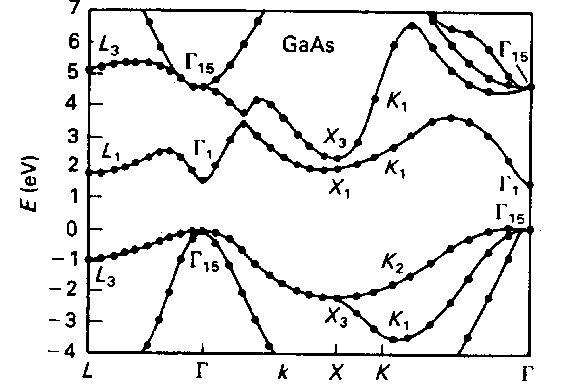
\includegraphics[width=0.5\textwidth]{Bilder/GaAs.png}
        \caption{Bandstruktur von GaAs \cite{BandstructureGaAs}.}
        \label{img:Bandstruktur}
    \end{figure}

    Für diesen Versuch ist die Bandlücke zwischen Valenz- und Leitungsband von besonderer Bedeutung
    Diese Bandlücke und die Fermi-Energie $E_\text{F}$ charakterisiert ein Material als Metall, Halbleiter oder Isolator.\\

    Metalle zeichnen sich durch ein vollständig gefülltes Valenzband und einige besetzte Niveaus im Leitungsband aus. Dies erlaubt es den Metallen, bei niedrigen Temperaturen elektrischen Strom zu leiten, da die Elektronen auf energetisch höhere Niveaus angeregt werden können und dadurch beweglicher sind.

Im Gegensatz dazu haben Halbleiter und Isolatoren ein komplett gefülltes Valenzband und ein unbesetztes Leitungsband, was ihnen keine Leitfähigkeit verleiht, da die Elektronen nicht in der Lage sind, ihre Niveaus zu wechseln. Bei Halbleitern ist jedoch die Bandlücke so gering, dass Elektronen bei erhöhten Temperaturen in das Leitungsband gelangen können, was das Material leitfähig macht.

Eine schematische Darstellung der Bandstruktur für verschiedene Materialien ist in \autoref{img:Band} dargestellt.


    \begin{figure}[H]
        \centering
        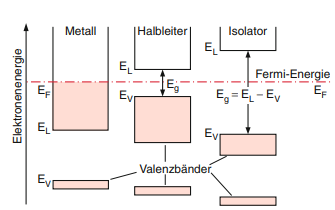
\includegraphics[width=0.6\textwidth]{Bilder/band.png}
        \caption{Beispielhafte Bandschemata von Metallen, Halbleitern und Isolatoren \cite{Demtröder}.}
        \label{img:Band}
    \end{figure}

    \subsection{Dotierung}

    Die Dotierung des Materials ermöglicht es, die Bandlücke zu modifizieren und somit die Leitfähigkeit zu beeinflussen. Es gibt zwei Arten der Dotierung: die n-Dotierung und die p-Dotierung.
Bei der n-Dotierung werden Donatoren, also Fremdatome mit einem zusätzlichen Valenzelektron, eingeführt. Diese Elektronen sind knapp unterhalb der Bandkante positioniert, was bedeutet, dass weniger thermische Energie benötigt wird, um sie ins Leitungsband zu verschieben. Dies kann zu einer signifikanten Leitfähigkeit bei Raumtemperatur führen.
Im Falle der p-Dotierung werden Akzeptoren, also Atome mit zusätzlichen Leerstellen, eingeführt. Das Energieniveau dieses Akzeptors liegt knapp oberhalb der Valenzbandkante. Der Übergang zu diesem Niveau erfordert weniger Energie, was zur Bildung einer Leerstelle im Valenzband führt und zur Lochleitfähigkeit beiträgt.
Die Niveaus dieser Dotierungen sind in den Abbildungen \autoref{img:dot1} und \autoref{img:dot2} dargestellt.

    \begin{figure}[H]
        \centering
        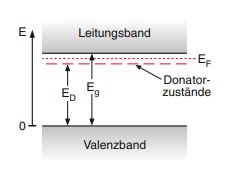
\includegraphics[width=0.4\textwidth]{Bilder/DonatorNiveau.png}
       \caption{Bandstruktur eines n-dotierten Halbleiters mit Fermi-Energie $E_{\text{F}}$ sowie Donatorniveau \cite{Demtröder}.}
        \label{img:dot1}
    \end{figure}

    \begin{figure}[H]
       \centering
       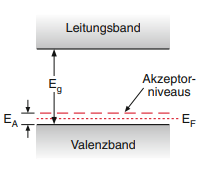
\includegraphics[width=0.4\textwidth]{Bilder/AkzeptorNiveau.png}
       \caption{Bandstruktur eines p-dotierten Halbleiters Akzeptorniveau und  $E_{\text{F}}$ \cite{Demtröder}.}
       \label{img:dot2}
   \end{figure}

    \subsection{Die effektive Masse}

    Um die Bewegung der Elektronen zu beschreiben, wird das Konzept der effektiven Masse $m^∗$ verwendet. Dieses Konzept berücksichtigt, dass die Elektronen nicht frei sind, sondern einem periodischen Potential unterliegen. Wenn sich die Elektronen in einem lokalen Minimum des Potentials befinden, kann ihre Beschleunigung gemäß dem zweiten Newtonschen Gesetz durch die Gleichung
    \begin{align*}
        a =\frac{1}{\hslash^2}\frac{\symup{d}^2\epsilon}{\symup{d}k^2} \cdot qE
    \end{align*}

    beschrieben werden, wobei $a$ die Beschleunigung, $q$ die Ladung des Elektrons und $E$ das externe elektrische Feld ist.
    Hieraus folgt mit $F=m^*a$

    \begin{equation}
    \label{eq:effektiveMasseeee}
        m^* =  \hbar^2 \frac{\symup{d}k^2}{\symup{d}^2\epsilon}\quad.
    \end{equation}

    Dass diese Annahme sinnvoll ist zeigt sich, da die Dispersionsrelation $\epsilon(k)$ in der Nähe eines Minimums durch eine Parabel angenähert werden kann.
    Eine Taylor-Entwicklung um das Minimum $\epsilon^{\prime}\left(k_0\right)=0$ in $k$ liefert

        \begin{align*}
            \epsilon(k) \approx \epsilon\left(k_0\right)+\epsilon^{\prime}\left(k_0\right)\left(k-k_0\right)+\frac{1}{2} \epsilon^{\prime \prime}\left(k_0\right)\left(k-k_0\right)^2=\epsilon\left(k_0\right)+\frac{1}{2} \epsilon^{\prime \prime}\left(k_0\right)\left(k-k_0\right)^2.
        \end{align*}

    Vereifacht mit $\epsilon_{k_0} = 0$ und $k_0 = 0$ ergibt sich

    \begin{align*}
        \epsilon(k) \approx \frac{1}{2} \epsilon^{\prime \prime}(0) k^2.
    \end{align*}

    Es ergibt sich also eine Parabel.
    Folglich ist die Verwendung der \autoref{eq:effektiveMasseeee} gerechtfertigt.\\

    In der Regel ist $m^*$ ein Tensor, da die effektive Masse richtungsabhängig sein kann.
    Bei isotropen Festkörperkristallen wird $m^*$ zu einem Skalar.

    \subsection{Zirkulare Doppelbrechung}

    Bei der zirkularen Doppelbrechung tritt ein linear polarisierter Lichtstrahl in ein Material ein und ändert nach Austritt
    den Polarisationswinkel. Zur Berechnung des Drehwinkels $\theta$ wird angenommen, dass die Lichtwelle durch eine Superposition aus einer rechts- und linkszirkulären Welle dargestellt werden kann.

    \begin{align}
    \label{eq:gl3}
    E(z)=\dfrac{1}{2}(E_\text{R}(z)+E_\text{L}(z))
    \end{align}

    Dabei sind die Phasengeschwindigkeiten der beiden Teilwellen des Lichtes im Material unterschiedlich.
    Durch Umformen und Zerlegen der \autoref{eq:gl3} kann folgender Ausdruck für den Drehwinkel $\theta$ ermittelt werden.

    \begin{align}
    \label{eq:gl4}
    \theta= \dfrac{d\omega}{2c} \left(\dfrac{1}{v_{\text{Ph}_R}}-\dfrac{1}{v_{\text{Ph}_L}}\right)
    \end{align}

    Mit Hilfe der Brechungsindizes $n_\text{R}$ und $n_\text{L}$ wird die \autoref{eq:gl4} zu

    \begin{align*}
    \theta= \dfrac{d\omega}{2} (n_\text{R}-n_\text{L})
    \end{align*}

    $L$ ist hierbei die Länge des Materials und $\omega$ die Kreisfrequenz der einfallenden Welle. 
    Die Doppelbrechung entsteht durch das elektrische Dipolmoment, das durch die Atome an den Gitterpositionen und durch die Interaktion der Bandelektronen mit den Atomkernen erzeugt wird. Die Summe der Dipole pro Volumeneinheit, die als mikroskopische Polarisation bekannt ist, beträgt

    \begin{align*}
    \vec{P}=\epsilon_0 \chi \vec{E}
    \end{align*}

     mit der dielektrische Suszeptibilität $\chi$. Bei isotroper Materie stellt dieser eine skalare Größe dar und bei anisotropen Kristallen
    einen Tensor dritter Stufe. Nach weiteren Umrechnungen erhält man für den Drehwinkel den Ausdruck

    \begin{align*}
    \theta= \dfrac{d\omega}{2cn}\chi_{xy}
    \end{align*}

    \newpage

    \subsection{Berechnung des Rotationswinkels beim Faraday Effekt}

    Der Faraday Effekt wird durch das Anlegen eines äußeren Magnetfeldes erzeugt.
    Dabei kommt es zu einer Wechselwirkung des Magnetfeldes mit den Elektronen des Festkörpers. Für ein gebundenes Elektron gilt die
    folgende Bewegungsgleichung

    \begin{align*}
    m\dfrac{d^2\vec{r}}{dt^2}+K\vec{r}=-e_0\vec{E}(r)-e_0\dfrac{d\vec{r}}{dt}\times\vec{B}
    \end{align*}

    mit der Elektronenmasse $m$ und der Elektronenladung $q$. Der Vektor $\vec{r}$ ist die Auslenkung aus dem Ruhezustand, $\vec{E}$ beschreibt die Feldstärke der es einfallenden Lichtes und $K$ ein konstanter Faktor der Rückstellkraft.
    Wenn nun der magnetische Teil der Lichtwelle neben Dämpfungseffekten vernachlässigt wird, da dieser ohnehin nur einen geringen Einfluss auf den Faraday-Effekt nimmt, folgt für den Winkel der Polarisationsebene mit
   

    \begin{align*}
    \vec{P}&=-Ne_0\vec{r} \quad \text{und}\\
    \chi_{xy}&=\dfrac{Ne_0^3\omega B}{\epsilon_0\left(\left(-m\omega^2+K\right)^2-\left(e_0\omega B\right)^2\right)}
    \end{align*}

    die wichtige Gleichung

    \begin{align}
    \label{eq:gl11}
    \theta=\dfrac{e_0^3}{2\epsilon_0 c}\dfrac{1}{m^2}\dfrac{\omega^2}{\left(-\omega^2+\dfrac{K}{m}\right)^2 -\left(\dfrac{e_0}{m}B\omega\right)^2}  \dfrac{NBd}{n}
    \end{align}

    mit der Flussdichte $B$, der Probenlänge $D$ und der Zahl der Ladungsträger $N$ pro Volumeneinheit. $\sqrt{\dfrac{K}{m}}$
    kann hier als Resonanzfrequenz $\omega_0$ und $\dfrac{Be_0}{m}$ als Zyklotron-Frequenz $\omega_C$ bezeichnet werden. 
    Unter der Annahme, dass die Messfrequenz viel kleiner als $\omega_0$ und dass die Resonanzfrequenz größer als die Zyklotron-Frequenz ist,
    lässt sich die \autoref{eq:gl11} umformen zu

    \begin{align*}
    \theta(\lambda)=\dfrac{2\pi^2 e_0^3 c}{\epsilon_0}\dfrac{1}{m^2}\dfrac{1}{\lambda^2 \omega_0^4}\dfrac{NBd}{n}\; .
    \end{align*}

    Für freie Ladungsträger ergibt sich mittels der Annahme, dass $\omega_0$ gegen Null geht

    \begin{align}
    \label{eq:gl12}
    \theta_{frei}=\dfrac{e_0^3\lambda^2}{8 \pi^2 \epsilon_0 c^3 m^2 }\dfrac{NBd}{n}\; .
    \end{align}

    Wird $m$ durch $m^*$ ersetzt, so erhält man den Zusammenhang zwischen Drehwinkel $\theta$ und der effektiven Masse $m^*$
    der Elektronen im Kristall.

    \newpage